\documentclass{article}
\title{Medical Faculty - Undergraduates  - Exam of Biostatistics}
\date{31.7.2013}
\usepackage[english]{babel}
\usepackage{enumerate}
\usepackage[cm,empty]{fullpage}
\usepackage[pdftex]{graphicx,color}
\usepackage{Sweave}
\begin{document}
\maketitle{}
\framebox{Name:\hspace{3cm}ID Number:\hspace{3cm}Points:\hspace{2cm}Exam831 }\begin{itemize}
\item[1] {\small $\left[5\right]$ }Which of the following is a measure of central tendency?
\begin{enumerate}[(a)]
\item mean 
{\bf T }\item range 
{\bf F }\item variance 
{\bf F }\item standard deviation 
{\bf F }\item coefficient of correlation 
{\bf F }\item mode 
{\bf T }\item median 
{\bf T }\item frequency 
{\bf F }\end{enumerate}
\item[2] {\small $\left[15\right]$ }A genetically modified mouse does not survive the first month of life with probability 0.40.  
\begin{enumerate}[(a)]
\item We planned an experiment that included 10 mice. What is the probability that after a month not more than a mouse will survive? 
{\bf $X=1$ survive, $P(X=1)=p=.6, Y=sum(X), P(Y<=1)=P(Y=0)+P(Y=1)=(1-p)^10+10*p(1-p)^9$ -> $P(Y<=1)= 0.0017$ }\vspace{\baselineskip} \vspace{\baselineskip}\item What is the expected number of mice still alive after the first month? 
{\bf $E(X)=pn -> E(X)=6$ }\vspace{\baselineskip}\end{enumerate}
\item[3] {\small $\left[15\right]$ }Data for variable nn are represented graphically.\\ 
\begin{tabular}{c}
\resizebox{50mm}{!}{
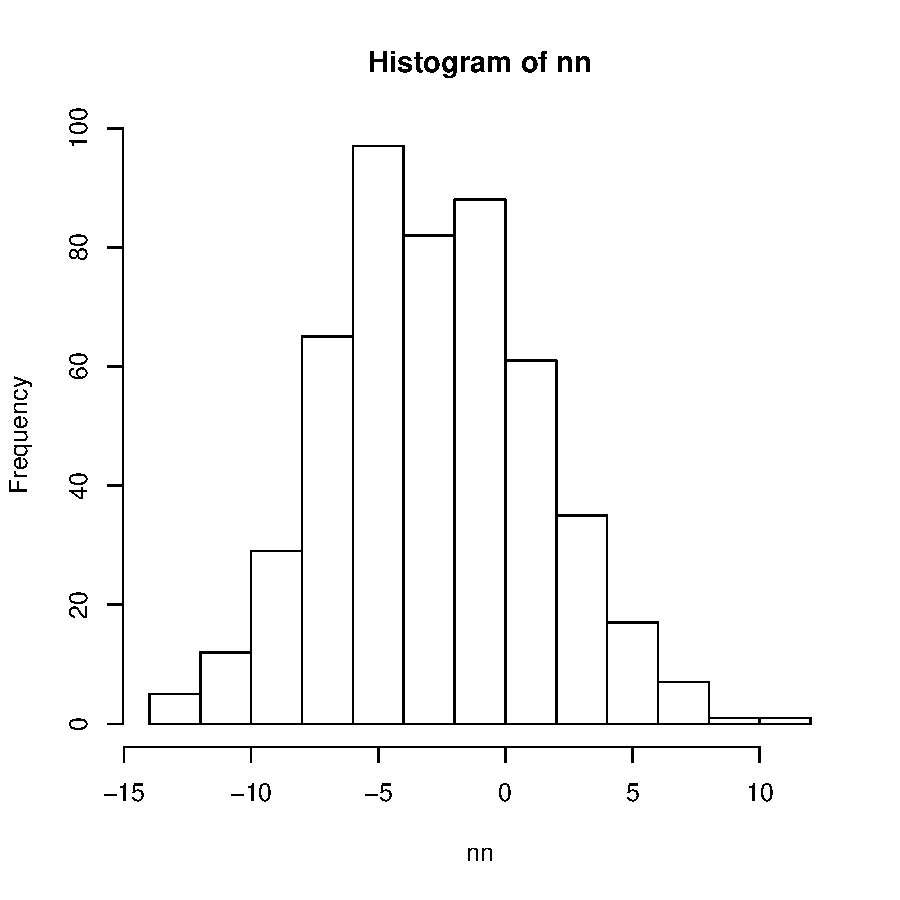
\includegraphics{Exam1sol-001}
}
\end{tabular}

\begin{enumerate}[(a)]
\item Is standard deviation 1, 2 or 4? 
{\bf 4 }\item Is mean -3, 0 or 3? 
{\bf -3 }\end{enumerate}
\item[4] {\small $\left[15\right]$ }
What is the probability of obtaining exactly 1 tails if we toss a fair coin 2 times?
{\bf 
 
Number of trials: n=2, Number of successes=k=1,  probability of success: p=0.5. Using binomial distribution: $P(X=k|n,p)=$0.75. }\vspace{\baselineskip} \vspace{\baselineskip} \vspace{\baselineskip}\end{itemize}
\newpage
\end{document}
